\documentclass[aspectratio=169]{beamer}
\usetheme{default}
\usecolortheme{seahorse}
\setbeamertemplate{navigation symbols}{}
\setbeamertemplate{footline}[frame number]
\usepackage{amsmath,amssymb,booktabs,graphicx}
\newcommand{\Ex}{\mathbb E}
\newcommand{\Prb}{\mathbb P}
\title{Sharp Guarantees for Ensemble Voting}
\subtitle{An elementary analysis of dependence --- DSAA2011 Project 2}
\author{Project team --- replace with actual members}
\date{}
\begin{document}
\begin{frame}\titlepage\end{frame}
\begin{frame}{The question and the contribution}
For $K=2m+1$ fixed binary classifiers, let $Z_i$ indicate correctness.
\[
S=\sum_iZ_i,\qquad A=\Prb(S\ge m+1).
\]
\begin{itemize}
\item What do marginals and correlations determine about $A$?
\item When must $A$ exceed the common member accuracy $p$?
\item Our focus: elementary sharp bounds, explicit attaining laws, and a finite-$K$ threshold.
\end{itemize}
\medskip
Sharp moment bounds and the insufficiency of pairwise information are classical. The project contributes a self-contained simplification and synthesis, not a claim of the first two-moment inequality.
\end{frame}
\begin{frame}{Part I: opposite behavior with and without independence}
\[
 A_{\rm ind}=\sum_{s=m+1}^K\binom Ks p^s(1-p)^{K-s},\qquad
 A_-^{\rm marg}=\max\left(0,\frac{Kp-m}{m+1}\right).
\]
For $p>1/2$, independent accuracy tends to $1$, whereas the worst marginal-only accuracy tends to $2p-1$.
\medskip

The lower bound follows from $S\le m+(m+1)\mathbf1\{S>m\}$.
It is attained using only counts $m,K$ when $Kp>m$.
\medskip

Unequal marginals: sort $p_{(1)}\ge\cdots\ge p_{(K)}$ and use
\[
\max\left(0,\max_{r\ge m+1}\frac{\sum_{i=1}^r p_{(i)}-m}{r-m}\right).
\]
Weights alone cannot improve the marginal-only minimax value beyond the best classifier.
\end{frame}
\begin{frame}{Part II: pairwise independence is not joint independence}
For $K=3$, common $p,r=\Ex Z_iZ_j$, write $q=\Prb(111)$.
\[
\max(0,2r-p)\le q\le\min(r,1-3p+3r),\quad A=3r-2q.
\]
At $p=0.6$, $r=0.36$ (every pair independent):
\begin{center}
\begin{tabular}{lrrrrr}\toprule
 & $Q_0$ & $Q_1$ & $Q_2$ & $Q_3$ & $A$\\\midrule
Worst & 0 & .48 & .24 & .28 & .52\\
Independent & .064 & .288 & .432 & .216 & .648\\
Best & .16 & 0 & .72 & .12 & .84\\\bottomrule
\end{tabular}
\end{center}
Conditional on $S=s$, choose the correct subset uniformly. This verifies every marginal and pairwise moment in the table.
\end{frame}
\begin{frame}{Replace $2^K$ configurations by one integer count}
With equal $p$ and equal $r$, randomly permuting voter indices preserves all constraints and the objective.
\[
\mu=\Ex S=Kp,\qquad \nu=\Ex S(S-1)=K(K-1)r.
\]
Conversely, uniform allocation within each count realizes every count law with these moments.
\medskip

The feasible moment region is the polygon through $(s,s(s-1))$, $s=0,\ldots,K$.
If $b=\lfloor\mu\rfloor$,
\[
2b\mu-b(b+1)\le\nu\le(K-1)\mu.
\]
This is a finite symmetrization argument, not an assumption of an infinite iid mixture.
\end{frame}
\begin{frame}{Two families of simple quadratic certificates}
For every integer $s\in[0,K]$, all these functions are at most $\mathbf1\{s>m\}$:
\[
0,\quad h(s)=\frac{s(s-m)}{K(K-m)},\quad
 g_j(s)=1-\frac{(s-j)(s-j-1)}{(j-m)(j+1-m)},\quad m+1\le j<K.
\]
\begin{itemize}
\item For $s\le m$, each function is nonpositive.
\item For $s>m$, $h(s)\le1$ and consecutive integers have nonnegative product, so $g_j(s)\le1$.
\item Taking expectations gives the exact lower bound $B_K$ by maximizing these certificates.
\end{itemize}
\medskip
The upper endpoint follows by complementing all votes: $S\mapsto K-S$.
\end{frame}
\begin{frame}{Why the bound is attained: a picture is enough}
\begin{columns}
\column{.56\textwidth}
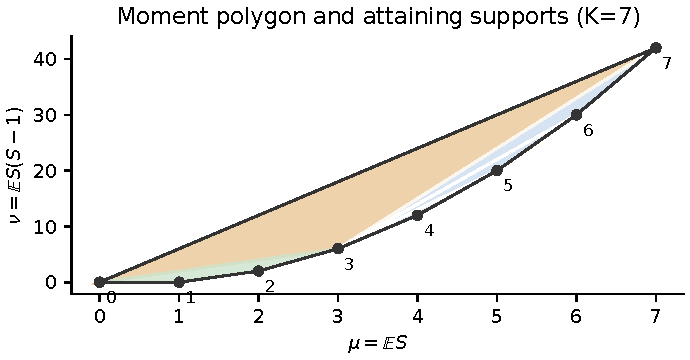
\includegraphics[width=\linewidth]{figures/moment_polygon.pdf}
\column{.43\textwidth}
\begin{itemize}
\item Green: losing counts only, so $A=0$.
\item Orange: support $\{0,m,K\}$ attains $h$.
\item Blue: support $\{m,j,j+1\}$ attains $g_j$.
\end{itemize}
Every feasible point lies in a piece. Its barycentric coordinates are the required probabilities. No general LP duality is needed.
\end{columns}
\end{frame}
\begin{frame}{A one-line comparison gives constant-time evaluation}
Set $d=\mu-m$, $v=\Ex(S-m)^2$, and $j=m+a$. Then
\[
G_a=\Ex g_{m+a}(S)=\frac{(2a+1)d-v}{a(a+1)},
\]
\[
G_a-G_{a+1}=\frac{2[(a+1)d-v]}{a(a+1)(a+2)}.
\]
If $d\le0$, every $G_a\le0$. Otherwise choose
\[
a_*=\operatorname{clip}(\lfloor v/d\rfloor,1,m).
\]
Only $0$, $\Ex h$, and $G_{a_*}$ need comparison. This is constant-time arithmetic given the two moments; it does not make reading a full pairwise matrix constant-time.
\end{frame}
\begin{frame}{The exact threshold for beating a member}
For $1/2<p<1$, define
\[
x=\frac{Kp-(1-p)m}{p},\quad j=\lfloor x\rfloor,\quad\theta=x-j,
\]
\[
\nu_*=(1-p)m(m-1)+p[2jx-j(j+1)],\quad
\rho_*=\frac{\nu_*/[K(K-1)]-p^2}{p(1-p)}.
\]
\begin{block}{Necessary and sufficient, within the feasible range}
\[ A_{\min}>p\quad\Longleftrightarrow\quad\rho<\rho_* .\]
\end{block}
At the boundary, put masses $1-p,p(1-\theta),p\theta$ on $m,j,j+1$.
Accuracy is exactly $p$. Mixing with synchronized votes covers every correlation above the threshold without improving accuracy.
\end{frame}
\begin{frame}{Separate the threshold correction from the integer correction}
\small
For $d=Kp-m$, the gain over the original C-bound threshold $\rho_C$ is
\[
\rho_*-\rho_C=
\underbrace{\frac{p-1/2+1/(4K)}{(K-1)p^2}}_{\text{correct failure threshold}}
+\underbrace{\frac{\theta(1-\theta)}{K(K-1)(1-p)}}_{\text{integer support}}.
\]
\centering
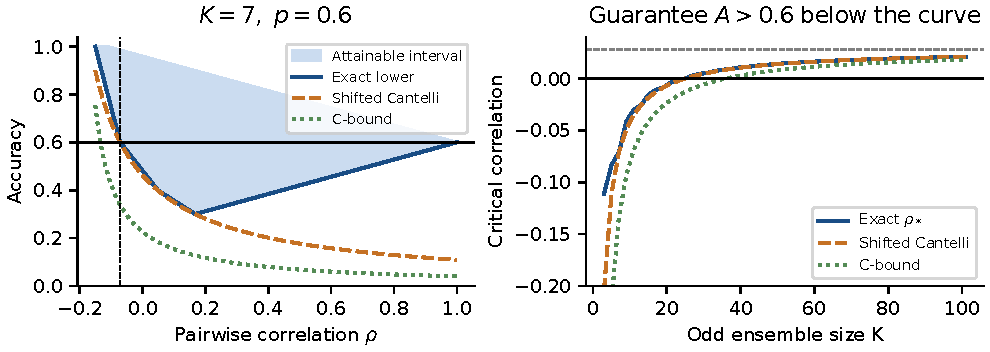
\includegraphics[width=.77\linewidth]{figures/bounds.pdf}
\end{frame}
\begin{frame}{A concrete consequence: 27 pairwise-independent voters}
For $p=3/5$, $\rho=0$, and $K=2m+1$,
\[
\rho_* = \frac{m-12+(5/m)\mathbf1\{3\nmid m\}}{18(2m+1)}.
\]
\begin{center}
\begin{tabular}{lrrr}\toprule
 & $K=23$ & $K=25$ & $K=27$\\\midrule
Exact worst accuracy & .592 & .600 & .616\\\bottomrule
\end{tabular}
\end{center}
\begin{itemize}
\item The first strict guaranteed gain is at odd $K=27$.
\item Original C-bound first certifies it at $37$.
\item Shifted Cantelli also first certifies it at $27$ in this example: the full improvement here is not a lattice effect.
\end{itemize}
\end{frame}
\begin{frame}{Verification and what the result does not assume}
\begin{itemize}
\item 702 count-LP cases; 41 full binary-LP cases; both endpoints checked.
\item 720 threshold cases; integer boundaries, degenerate marginals, and attaining laws checked.
\item Largest count-LP discrepancy below $3\times10^{-14}$.
\item Proofs establish sharpness; experiments check implementations.
\item Unequal pairwise constraints still use the general LP. Estimated moments require uncertainty regions.
\end{itemize}
\medskip
\textbf{Takeaway:} pairwise information may not identify accuracy, yet it can certify an improvement. The integer count support makes that certification exact and elementary.
\end{frame}
\begin{frame}{References and preparation for Q\&A}
\footnotesize
Kuncheva \& Whitaker (2003), \emph{Measures of diversity}; Kuncheva et al. (2003), \emph{Limits on majority vote accuracy}.\\[.4em]
Germain et al. (2015), \emph{Risk bounds for the majority vote}, Theorem 11 and Proposition 13.\\[.4em]
Masegosa et al. (2020), \emph{Second order PAC-Bayesian bounds}, Theorems 3 and 6.\\[.4em]
Bertsimas \& Popescu (2005), \emph{Optimal inequalities in probability theory}; Boros \& Pr\'ekopa (1989), \emph{Closed form two-sided bounds}; Fontana \& Semeraro (2021), arXiv:2101.07693.\\[1em]
Prepare to explain: why symmetrization is lossless, why the quadratics work only on integers, why the three-point law attains the threshold, and why population guarantees do not imply finite-sample confidence.\\[.7em]
AI assistance: OpenAI Codex supported reading, derivation, code, and drafting. Team names and accurate individual contributions must be completed before submission.
\end{frame}
\end{document}
